\section{Empirical Evaluation} \label{Sec:evaluation}

To quantitatively assess the efficacy of our mutation testing approach, we have conducted a case study in which we address the following research questions:

\begin{description}
\item [RQ1] How efficient is \mutandis in generating non-equivalent mutants?
%\item [RQ2] How effective is \codename in injecting critical behaviour-affecting faults?
\item [RQ2] How effective are $FunctionRank$ and selective variable mutation in (i) generating non-equivalent mutants, and (ii) injecting non-trivial behaviour-affecting faults?
\item [RQ3] How useful is \mutandis in assessing the existing test cases of a given application?

\end{description} 

The experimental data produced by \mutandis is available for download.\footnoterecall{mutandisDownload}

\begin{table*}
\centering
%\vspace{5pt}
        \caption{Characteristics of the experimental objects.}
{\scriptsize
    \begin{center}
       
      %  \subtable[Experimental subjects and the corresponding exploration data]
            {
           \begin{tabular}{c|l|c|c|c|l} \hline
\theadturn{App ID} &\theadturn{Name} &\theadturn{JS LOC} & \theadturn{\# Functions} &\theadturn{CC} &\thead{Resource}  \\  \hline \hline

1  & SameGame & 206 & 9 & 37 & \url{http://crawljax.com/same-game}   \\ \hline
           
2 & Tunnel & 334 & 32  & 39 & \url{http://arcade.christianmontoya.com/tunnel} \\ \hline

3 & GhostBusters & 277 & 27 & 52 & \url{http://10k.aneventapart.com/2/Uploads/657}  \\ \hline

4 & Symbol & 204 &  20 & 32  & \url{http://10k.aneventapart.com/2/Uploads/652}\\ \hline

5 & TuduList & 2767 &  229 & 28  & \url{http://tudu.ess.ch/tudu}\\ \hline

6 & SimpleCart (library) & 1702 & 23  &  168 & \url{http://simplecartjs.org}\\ \hline

7 & \jquery (library)& 8371  &  45 & 37  & \url{https://github.com/jquery/jquery}\\ \hline

8 & WymEditor & 3035  &  188 & 50  & \url{https://github.com/wymeditor}\\ \hline

\hline\end{tabular}\centering
            }
\label{Table:objectsChar-table}
\end{center}
}  
\vspace{-0.1in} 
\end{table*}


\subsection{Experimental Objects}
Our study includes eight \javascript-based objects in total. Four
are game applications, namely, SameGame, Tunnel, GhostBusters, and Symbol. One is  a web-based task management application called TuduList. Two, namely SimpleCart and \jquery, are \javascript libraries. The last application, WymEditor, is a web-based HTML editor. All the experimental objects are open-source applications.
One of our main inclusion criteria was for the applications to extensively use \javascript on the client-side.
Although the game applications used in our study are small size web applications, they all extensively and in many different ways use \javascript.

%
\tabref{objectsChar-table} presents each application's ID, name, and resource, as well as the static  characteristics of the \javascript code, such as \javascript lines of code (LOC) excluding libraries, number of functions, and the cyclomatic complexity (CC) across all \javascript functions in each application.

\begin{table}
%\vspace{5pt}
        \caption{Bug severity description.}
{\scriptsize
    \begin{center}
       
      %  \subtable[Experimental subjects and the corresponding exploration data]
            {
           \begin{tabular}{l|l|l} \hline
\thead{Bug Severity} &\thead{Description} &\thead{Rank}  \\  \hline \hline

Critical  & Crashes, data loss & 5   \\ \hline
Major  & Major loss of functionality & 4   \\ \hline
Normal  & Some loss of functionality, regular issues & 3   \\ \hline
Minor  & Minor loss of functionality & 2   \\ \hline
Trivial  & Cosmetic issue & 1   \\ \hline

\hline\end{tabular}\centering
            }
\label{Table:bugSeverity-table}
\end{center}
}  
\vspace{-0.1in} 
\end{table} 


\subsection{Experimental Setup}
To run the analysis, we provide the URL of each experimental object to \mutandis. 
Note that because SimpleCart and \jquery are both \javascript libraries, they cannot be executed independently. However, since they come with test cases, we use them to answer RQ3.
%we are not able to use them in response to RQ1 and RQ2, as they are not independently executable. 
%As a result, we use them to answer RQ4. %The first five applications are used for answering RQ1--RQ3.

We evaluate the efficiency of \mutandis in generating non-equivalent mutants (\textbf{RQ1}) for the first five applications in \tabref{objectsChar-table}. 
We collect execution traces by instrumenting the custom \javascript code of each application and executing the instrumented code through automated dynamic crawling. 
We navigate each application several times with different crawling settings. Crawling settings differ in the number of visited states, depth of crawling, and clickable element types.
We inject a single fault at a time in each of these five applications using \mutandis. The number of injected faults for each application is 40; in total, we inject 200 faults for the five objects. We automatically generate these mutants from the following mutation categories: (1) variables, (2) branch statements, and (3) \javascript-specific operators. We then examine each application's behaviour to determine whether the generated mutants are equivalent.  

The determination of whether the mutant is equivalent is semi-automated for observable changes.
An observable change is a change in the behaviour of the application which can be observed as the application is automatically executed in the browser.
Note that in web applications DOM is an observable unit of the application, which is shown in the browser. We execute the same sequence of events in the mutated version as it is used in the original version of the application. The resulting observable DOM of the mutated version in the browser is visually compared against the original version. 
%as we automatically execute the mutated version of the application in the browser. 
If we notice any observable change during the execution, the mutant is marked as non-equivalent. 
This way we can eliminate the burden of manual analysis of the applications' source code for every mutants.  
For non-observable changes, we manually inspect the application's source code to determine whether the mutant is equivalent.
%\karthik{How is executing the application in the browser enough to detect observable changes ? Do we not need someone to observe the difference ?}

To make sure that changes in the applications' behaviour, from which the non-equivalency is determined, are not cosmetic changes we use the bug severity ranks used by Bugzilla, a popular bug
tracking system. %which have also been used by other researchers \cite{bhattacharya:icse12}. 
The description and the rank associated with each type of bug severity is shown in \tabref{bugSeverity-table}. We choose non-equivalent mutants from our previously generated mutants (for RQ1). We then analyze the output of the mutated version of the application and assign a bug score according to the ranks in \tabref{bugSeverity-table}.

To address \textbf{RQ2}, we measure the effectiveness of \mutandis in comparison with random-based mutation generation. Moreover, to understand the impact of applying $FunctionRank$ and rank-based variable mutation in generating non-equivalent mutants as well as injecting behaviour-affecting faults we compare:
\begin{enumerate} [noitemsep, nolistsep]
\item The proposed $FunctionRank$ metric with $PageRank$;
\item Our selective variable mutation with random variable mutation;
\end{enumerate}
Similar to RQ1, we use the ranks provided by Bugzilla to measure the criticality of the injected faults on the non-equivalent mutants.  

Unfortunately, no test suites are available for the first five applications.  Thus, to address \textbf{RQ3}, we run our tool on the SimpleCart, \jquery, and WymEditor that come with Qunit\curl{http://docs.jquery.com/QUnit} test cases. We gather the required execution traces of the SimpleCart library by running its test cases, as this library has not been deployed
on a publicly available application. However, to collect dynamic traces of the \jquery library, we use one of our experimental objects (SameGame), which uses \jquery as one of its \javascript libraries. Unlike the earlier case, we include the \jquery library in the instrumentation step. We then analyze how the application uses different functionalities of the \jquery library using our approach. The execution traces of the WymEditor are collected by crawling the application. We generate 120 mutants for each of the three experimental objects. Mutated statements, which are not executed by the test suite are excluded. After injecting a fault using \mutandis, we run the test cases on the mutated version of each application. 
We determine the usefulness of our approach based on (1) the number of non-equivalent generated mutants, and (2) the number of non-equivalent \emph{surviving} mutants.  A non-equivalent surviving mutant  is one that is neither killed nor equivalent, and is an indication of the incompleteness of the test
cases. The presence of such mutants can help testers to improve the quality of their test suite. 
For mature test suites, we expect the number of non-equivalent surviving mutants to be low \cite{raise:jalbert12}. We further compare \mutandis against random mutation testing to evaluate the effect of our approach on the stubbornness of the generated mutants. Stubborn mutants are non-equivalent mutants that remain undetected by a high quality test suite \cite{yao:icse14}.

\begin{table*}
%\vspace{5pt}
        \caption{Mutants generated by \mutandis.}
{\scriptsize
   
       \begin{center}
      %  \subtable[Experimental subjects and the corresponding exploration data]
            {
          \begin{tabular}{l|l|l|l|l|l|l} \hline
\thead{Name} & \thead{\# Mutants} & \thead{\# Equiv Mutants} & \thead{\# Non-Equiv Mutants} & \thead{Equiv Mutants (\%)} & \thead{Bug Severity Rank (avg)} & \thead{Bug Severity (\%)} \\  \hline \hline

  SameGame & 40 & 2 & 38 & 5.0 & 3.9 & 78\\ \hline
  Tunnel & 40 & 4 & 36 & 10.0 & 3.8 & 76\\ \hline
  GhostBusters & 40 & 3 & 37 & 7.5 & 3.2 & 64\\ \hline
  Symbol & 40 & 3 & 37 & 7.5 & 3.9 & 78 \\ \hline
  TuduList & 40 & 2 & 38 & 5.0 & 3.8 & 76\\ \hline 
 Avg. & 40 & 2.8  & 37.2  & 7.0 & 3.7  & 74.4 \\ \hline
  

\hline \end{tabular}\centering
            }

\label{Table:bugSeverity-equiv-table}
\end{center}
}  
\vspace{-0.1in} 
\end{table*}

\subsection{Results}
%In this section, we discuss the results of the case study with regard to our three research questions.
\head{Generated Non-Equivalent Mutants (RQ1)} \tabref{bugSeverity-equiv-table} presents our results for the number of non-equivalent mutants and the severity of the injected faults using \mutandis.
For each web application, the table shows the number of mutants, number of equivalent mutants, the number of non-equivalent mutants, 
the percentage of equivalent mutants, and the average bug severity as well as the percentage of the severity in terms of the maximum severity level. 
%$\left(\frac{\#Non-EquivMutants}{\#TotalMutants}\right)\times 100$

As shown in the table, the number of equivalent mutants varies between 2--4, which corresponds to less than 10\% of the total number of mutants.%, which compares favourably to other techniques that have observed the number of equivalent mutants to be between 10 to 40\%.

\answer{On average, the percentage of equivalent mutants generated by \mutandis is  7\%, which points to its efficiency in generating non-equivalent mutants.} 

We observe that more than 70\% of these equivalent mutants generated by \mutandis originate from the branch mutation category. The reason is that in our current approach, branch expressions are essentially ranked according to the variables used in their expressions without considering whether mutating the expression changes the actual boolean outcome of the whole expression (e.g.; \code{if(trueVar || var)\{...\}} where the value of \code{trueVar} is always \code{true}, and thus mutating \code{var} to \code{!var} does not affect the boolean outcome of the expression). We further notice cases in our experimental objects where the programmer writes essentially unused hard-coded branch expressions.
%This can result in mutating a branch that does not affect the application's behaviour. 
For instance, in Tunnel, we observed a couple of \code{return true/false} statements at exit point of the functions that have high $FunctionRank$ and cyclomatic complexity value. However, the returned value is never used by the caller function and hence, mutating the return boolean value as part of branch mutation generates an equivalent mutant. This is the main reason that we observe 10\% of equivalent mutants (the highest in \tabref{bugSeverity-equiv-table}) for the Tunnel application. Moreover, we notice that certain types of mutation operators affect the number of equivalent mutants. For example for a number of mutations we observe that replacing $>=$ ($<=$) sign with $>$ ($<$) keeps the program's behaviour unchanged since either the lower/upper bound is never reached or the programmer specify extra bounds checking before returning the final value.
  
%As far as RQ1 is concerned
%our tool is capable of automatically generating mutants, which are not equivalent with high probability.
\headbf{Fault Severity of the Generated Mutants} The fault severity of the injected faults
is also presented in \tabref{bugSeverity-equiv-table}. We computed the percentage of the bug severity as the ratio of the average severity rank to the maximum severity rank (which is 5). As shown in the table, the average bug severity rank across all applications is 3.72 (bug severity percentage is 74.4\% on average).
%This indicates that the injected faults cause normal to major loss of functionality.
%Based on \tabref{bugSeverity-table}, we see that: 
%
%\answer{Based on an average severity rank of 3.72, the injected faults cause normal to major loss of functionality.}
%
We observed only a few faults with trivial severity (e.g; cosmetic changes).
We also noticed a few critical faults (3.8\% on average), which caused the web application to terminate prematurely or unexpectedly.
It is worth noting that full crashes are not that common for web applications, since web browsers typically do not stop executing the entire web application when an error occurs. The other executable parts of the application continue to run in the browser in response to user events \cite{Ocariza-2011}. 
Therefore, it is very rare for web applications to have type 5 errors, and hence the maximum severity rank is often 4.
%Further, we made the following important observation for all the applications:

\answer{More than 70\% of the injected faults causing normal to major loss of functionality are in the top 20\% ranked functions, showing the importance of $FunctionRank$ in the fault seeding process.}

Moreover, we noticed that the careful choice of a variable for mutation is also as important as the function selection. For example, in the SameGame
application, the \code{updateBoard} function is responsible for redrawing the game board each time a cell is clicked. Although \code{updateBoard}
is ranked as an important function according to its $FunctionRank$, there are two variables within this function that have
high usage frequency compared to other variables. While mutating either of these variables causes major loss of functionality, 
selecting the remaining ones for mutation either has no effect or only marginal effect on the application's behaviour.
Furthermore, we observed that the impact of mutating variables that are part of the invariants as well as the variables 
with high usage frequency can severely affect the application's behaviour. This indicates that both invariants and usage
frequency play a prominent role in generating faults that cause major loss of functionality, thereby justifying our choice
of these two metrics for variable selection (Section~\ref{variable-ranking}).   
%
%As far as RQ2 is concerned, our results indicate that \mutandis is effective in generating mutants that cause non-trivial errors in \javascript applications.


\begin{figure}[!t]
  \centering
  \includegraphics[width=0.7\hsize]{r-scripts/equivMuts-barPlot}
  \vspace{0.09in} 
  \mycaption{Equivalent Mutants (\%) generated by \mutandis, random, PageRank, and random variable selection.}
  \label{Fig:equivMuts-barPlot}
\end{figure}

\begin{figure}[!t]
  \centering
  \includegraphics[width=0.7\hsize]{r-scripts/bugSeverity-barPlot}
  \vspace{0.09in} 
  \mycaption{Bug Severity Rankd (Avg) achieved by \mutandis, random, PageRank, and random variable selection.}
  \label{Fig:bugSeverity-barPlot}
\end{figure}

\head{Effectiveness of $FunctionRank$ and selective variable mutation (RQ2)} \label{Sec:eval-comparison}

The results obtained from \mutandis, random mutation, $PageRank$, and random variable mutation %(1) \mutandis with random mutation, (2) $FunctionRank$ with $PageRank$, and (3) selective variable mutation with random  variable mutation, 
 in terms of the percentage of equivalent mutants and bug severity rank are shown in \figref{equivMuts-barPlot} and \figref{bugSeverity-barPlot}, respectively.



As shown in \figref{equivMuts-barPlot}, the percentage of equivalent mutants generated by \mutandis is always less than or equal to the ones generated by the other three approaches. 
Not surprisingly, random mutation obtains the largest percentage of equivalent mutants (ranges from 7.5--15\%). 
This indicates that our selective variable mutation plays a more prominent role in reducing the percentage of equivalent mutants generated by \mutandis.


\answer{On average, \mutandis reduces the number of equivalent mutants by 39\% in comparison with random mutation generation.}

\answer{On average, $FunctionRank$ and selective variable mutation reduce the number of equivalent mutants by 12\% and 26\%, respectively when compared with $PageRank$ and random variable mutation.}

We observed that for three applications (ID=1, 2, 4) the main reason behind the reduction in the number of equivalent mutants is the use of selective variable mutation, 
as by replacing selective variable mutation with random mutation,
the percentage of equivalent mutants significantly increases (ranges from 33--50\% increment)
For these applications, we observed that although high rank functions are selected for mutation, modifying a non-behavioural affecting part of the selected function's code (\ie a useless branch or variable) results in generating an equivalent mutant. Therefore, the choice of the variable or branch to mutate is very important.

However, for application with ID 3 (GhostBusters), $FunctionRank$ plays a prominent role in reducing the number of equivalent mutants.
\figref{equivMuts-barPlot} shows that for this application the percentage of equivalent mutants becomes the same as \mutandis, when we use random variable mutation coupled with $FunctionRank$. 
We observed that in the aforementioned application,
major variables in the program have high usage frequency. Moreover, these variables are shared among detected invariants, thus making the selection of a specific variable for mutation less
effective compared to other applications. For the last application (ID 5), we observed that $FunctionRank$ and selective variable mutation are both effective in terms of generating
non-equivalent mutants.

\figref{bugSeverity-barPlot} compares the severity of the injected faults according to the ranks provided in \tabref{bugSeverity-table}. The results show that \mutandis achieves the highest rank among the other approaches. Our mutation generation technique increases the criticality of the injected faults by 20\% in comparison with random mutation approach. 
%
%\answer{Our approach increases the criticality of the injected faults by 20\% in comparison with random mutation approach.}

We observed that by replacing $FunctionRank$ with $PageRank$, the severity of the behaviour-affecting faults drops by 13\%, which indicates that $FunctionRank$ outperforms $PageRank$ in terms of its impact on the behaviour of the application towards more critical failures.
%
%\answer{$FunctionRank$ outperforms $PageRank$ in terms of its impact on the behaviour of the application towards more critical failures.} 

We further noticed that using the proposed selective variable mutation increases the bug severity by 9\% on average. While this indicates the importance of
using the proposed variable mutation technique, it reveals that our rank-based function selection technique plays a more prominent role in increasing the severity degree of the injected faults compared to our variable selection strategy.
For example, in application with ID 2 (Tunnel), function \code{updateTunnel} contains the main logic of the application, and it is among the top-ranked functions.
Since \code{updateTunnel} is significantly used throughout the application' execution as its high rank indicates, modifications to the variables of the function affects the expected behaviour of the application, and cause the application to show more severe bugs. Our function ranking technique is able to guide the mutation process towards selecting \code{updateTunnel} function, and thus increasing the overall bug severity degree. 
On the other hand, more than 90\% of the local and global variables used in function \code{updateTunnel} are involved with crucial reading and writing of properties. While mutating such important variables generates non-equivalent mutants, it will not significantly improve the criticality of the injected faults \emph{among the non-equivalent mutants} compared to random selection of variables. This implies that
our variable selection strategy plays a more prominent role in generating non-equivalent mutants rather than increasing the severity degree of the mutation.       
       
\begin{table*}
%\vspace{5pt}
        \caption{Mutation score computed for SimpleCart, \jquery, and WymEditor.}
{\scriptsize
   
       \begin{center}
      %  \subtable[Experimental subjects and the corresponding exploration data]
            {
          \begin{tabular}{c|r|r|r|r|r|r|r|r|r|r||r|r|r|r|r|r|r} \hline
& & & & \multicolumn{7}{c||}{\thead{Mutandis}} & \multicolumn{7}{c}{\thead{Random}}\\
\cline{5-18}

 \theadturn{Name} & \theadturn{\# JS Test Cases} & \theadturn{JS Branch Coverage (\%)} & \theadturn{\# TotalMutants} & \theadturn{\# Equiv.} & \theadturn{\# Non-Equiv.} & \theadturn{\# Killed} & \theadturn{Non-Equiv. (\%)} & \theadturn{Equiv. (\%)}
& \theadturn{Non-Equiv. Surviving (\%)} & \theadturn{Mutation Score (\%)} & \theadturn{\# Equiv.} & \theadturn{\# Non-Equiv.} & \theadturn{\# Killed} & \theadturn{Non-Equiv. (\%)} & \theadturn{Equiv. (\%)}
& \theadturn{Non-Equiv. Surviving (\%)} & \theadturn{Mutation Score (\%)} \\  \hline \hline

  SimpleCart & 83 & 41 & 120 & 2 & 118 & 80 & 95 & 5 & 32 & 67 & 8 & 112 & 78 & 81 & 19 & 30 & 70\\ \hline
  JQuery & 644 & 73 & 120 & 3 & 117 & 106 & 79 & 21 & 9 & 90 & 6 & 114 & 107 & 54 & 46 & 6 & 94 \\ \hline
  WymEditor & 253 & 71 & 120 & 6 & 114 & 97 & 74 & 26 & 15 & 85 & 9 & 111 & 99 & 57 & 43 & 11 & 89\\ \hline


\hline \end{tabular}\centering
            }

\label{Table:mutationScore-table}
\vspace{-0.1in} 
\end{center}
}  
\vspace{-0.1in} 
\end{table*}

\head{Assessing Existing Test Cases (RQ3)} %\shabnam{This section includes our response to several questions asked by reviewer 2 and 3} 
The results obtained from analyzing the mutants generated by \mutandis on the test cases of SimpleCart, \jquery library, and WymEditor are presented in \tabref{mutationScore-table}. The columns under ``\mutandis'', and ``Random'' present the results obtained by using our approach and random mutation generation respectively. The table shows the number of test cases, branch coverage achieved by the test suite, number of mutants, number of equivalent mutants, number of non-equivalent mutants, number of mutants detected by the test suite (killed mutants), 
the percentage of non-equivalent mutants and the equivalent mutants, 
the percentage of non-equivalent surviving mutants, and the mutation score.
To compute the percentage of equivalent mutants in presence of the test suite, we follow the guidance suggested by \cite{schuler:tvr12}, where, $Equiv (\%)=\frac{\#Equiv}{\#TotalMutants-\#Killed} \times 100$. 
Similarly, the percentage of non-equivalent mutants is: $Non\mhyphen Equiv (\%)=\frac{\#Non\mhyphen Equiv}{\#TotalMutants-\#Killed} \times 100$
The percentage of non-equivalent surviving mutants is: $\frac{\#NonEquivSurvivingMutants}{\#TotalNonEquivMutants} \times 100$.

Mutation score is used to measure the effectiveness of a test suite in terms of its ability
to detect faults \cite{woodward:ist93}. The mutation score is computed according to the following formula: 
$\left(\frac{K}{M-E}\right) \times 100$, where $K$ is the number of killed mutants, $M$ is the  number of mutants, and $E$ is the number of equivalent mutants.    

\headbf{Quality of test suites} The test suites of both JQuery and WymEditor are frequently updated in response to issues raised by the users. Both JQUery and WymEditor have around 71\% branch coverage. This points to the overall high quality of the test cases considering how difficult it is to write unit-level test cases for \javascript code. 
Note that despite the low branch coverage of SimpleCart, we gather execution traces of this application based on the available test suite. Therefore, the process of mutation generation is performed according to the executed part of the application from the test suite point of view. We also observed that for the three applications in \tabref{mutationScore-table}, a substantial percentage of uncovered branches are related to check for different browser settings (\ie running the application under IE, FireFox, etc).

\headbf{Surviving mutants} As shown in the table, less than 30\% of the mutants generated by \mutandis are equivalent. 
SimpleCart achieves a mutation score of 67, which means there is much room for test case improvement in this application. 
For SimpleCart, we noticed that the number of non-equivalent, surviving mutants in the branch mutation category is more than twice the number in the variable mutation category. 
This shows that the test suite was not able to adequately examine several different branches in the SimpleCart library, possibly because it has a high cyclomatic complexity (\tabref{objectsChar-table}).
On the other hand, the QUnit test suite of the \jquery library achieves a high mutation score of over 90\%, which indicates the high quality of the designed test cases. However, even in this case, 9\% of the non-equivalent mutants are not detected by this test suite.

We further observed that:

\answer{More than 75\% of the surviving non-equivalent mutants are in the top 30\% of the  ranked functions.} 

This again points to the importance of $FunctionRank$ in test case adequacy assessment. %Note that for SimpleCart and \jquery, each function is selected at least once for the purpose of mutation. As far as WymEditor is concerned, around 5\% of the selected functions are among the least important functions from the $FunctionRank$ point of view. 

As far as RQ3 is concerned: 

\answer{\mutandis is able to guide testers towards designing test cases for important portions of the code from the application's behaviour point of view.}

\headbf{Stubbornness of the generated mutants} Comparing the percentage of equivalent mutants as well as surviving non-equivalent mutants generated by \mutandis to those generated by random mutation in \tabref{mutationScore-table}, reveals that while our approach decreases the percentage of equivalent mutants (55\% on average), it \emph{does not negatively affect the stubbornness of the mutants}. To better show the effectiveness of \mutandis in decreasing the number of equivalent mutants, we compute odds ratio, which is a useful measure of effect size for categorical data \cite{madeyski:tse13}; the odds of non-equivalent mutants generated by approach $M$ is computed as 
$odds_{Non\mhyphen Equiv\: in\: M}=\frac{\#Non\mhyphen Equiv_{M}-\#killed_{M}}{\#Equiv_{M}}$.

Regarding our results, $odds\: ratio_{Non\mhyphen Equiv}=\frac{odds_{Non\mhyphen Equiv\: in\: Mutandis}}{odds_{Non\mhyphen Equiv\: in\: Random}}=2.6$, which is the odds of non-equivalent mutants generated by \mutandis divided by the odds of non-equivalent mutants using random mutation generation. This indicates that the odds of non-equivalent
mutants generated by \mutandis is 2.6 times higher than the random mutation strategy. We similarly measure the $odds\: ratio_{killed}$ for the number of killed mutants. The $odds\: ratio_{killed}$ of 0.98 indicates that compared with random mutation generation, our approach does not sacrifice stubbornness of the mutants. We further discuss the stubbornness of the mutants in \secref{discussion}.          


\section{Discussion}
\label{Sec:discussion}

% \head{Correlation.} To examine the relationship between the 
% cyclomatic complexity of objects and the number of unique invariants, 
% we used R \cite{?} to calculate the non-parametric
% Spearman correlation coefficients (r) as well as the p-values (p), 
% and plotted the graphs. We present the combinations that
% indicate a possible correlation.\figref{inv-cc} depicts the scatter plot of the
% cyclomatic complexity versus the number of unique invariants. 
% The correlation coefficient ($r = 0.867$, $p = 0.002$) suggests that variables 
% are positively co-related: The higher the cyclomatic complexity, the more unique invariants
% are detected in the application. The reason might be that larger value of cyclomatic complexity 
% implies that more number of decision points are present in the program. Consequently, pushing more 
% restrictions on varibales and parameters of the application may result in inferring more number of
% invariants. 
% \begin{figure}
% \centering
% 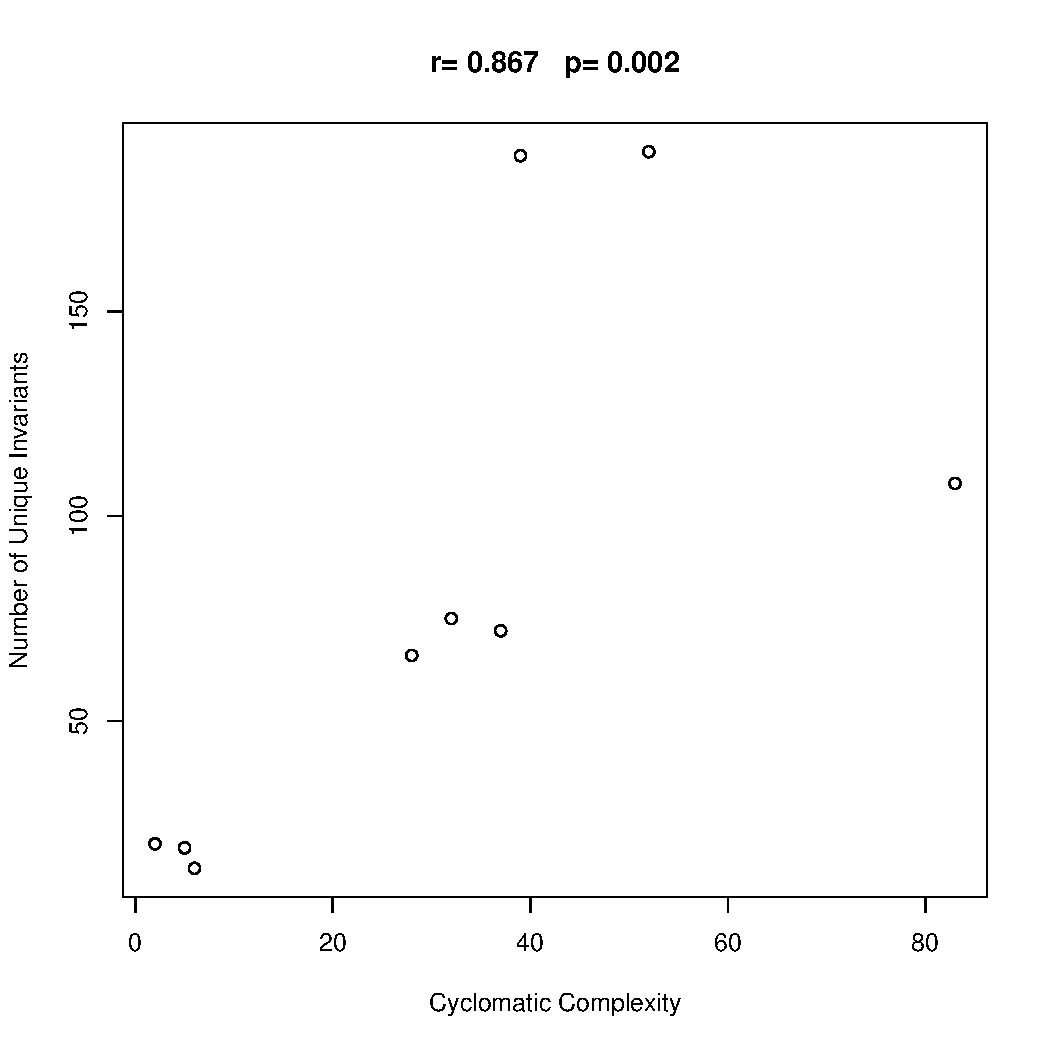
\includegraphics[width=0.7\hsize]{rscripts/inv_cc}
% \mycaption{Scatter plot of the number of unique invariants versus
% cyclomatic complexity. r represents the Spearman correlation coefficient and p is
% the p-value.}
% \label{Fig:inv-cc}
% \vspace{-0.3in}
% \end{figure}
%(1) the precision of comparing two floating point numbers in Daikon;
%The first is concerned with the number of digits in the fractional part of the floating point numbers, which is used by Daikon while comparing two floats. We resolve this by increasing the precision of float comparisons in Daikon configurations.
\head{Unstable Assertions.} As mentioned in \secref{filtering}, we observe a few number of unstable invariant assertions initially, which are removed by our filtering mechanism. By analyzing our trace data, we observe
that such unstable assertions arise mainly because of the 
multiple runtime types of \javascript variables.
This is based on the fact that in \javascript it is possible to change the type of a variable at runtime. However, Daikon treats variables as single type, selects the first observed type, and ignores the subsequent types in the trace data. This results in producing a few number of unstable invariant assertions for \javascript.
We remove such unstable assertions in our filtering step. A drawback of removing these assertions, is that our tool might miss a fault during the regression testing phase.
However, according to our observations, such unstable assertions form only around 5\% of the total generated assertions. Thus, we are still able to achieve high accuracy as presented in the previous section.
    
\head{Limitations.} Our approach is not able to detect syntax errors that are present in the \javascript code. Furthermore, tracing DOM manipulations using APIs other than the standard DOM API or jQuery is currently not supported by \jsart.
Further, a regression fault either directly violates an invariant assertion, or it can violate closely 
related assertions, which have been affected by the fault. However, if the tool is not able to infer any invariants in the  affected scope of the error, it fails to detect the fault. This results in observing a low rate of false negatives as illustrated in \secref{evaluation}. 
     
\head{Revisiting the Assumptions.} As we mentioned in \secref{approach}, we assume that the current version of the web application is bug-free. This is based on the fact that in regression testing a gold standard is always needed as a trusted version for comparing the test results against \cite{Binder:2000} to detect regression faults. However, if the original version of the application does contain an error, the generated assertions might reflect the error as well, and as such they are not able to detect the fault. 
Our second assumption states that the program specifications are unlikely to change frequently in revisions. Here we assume that software programs evolve gradually and regression faults are mostly due to small changes. However, if major upgrades occur in subsequent revisions such that the core specification of the application is affected, the inferred invariants from the original version may not be valid any longer and new invariant assertions need to be generated.

% Competent Programmer Hypothesis (CPH) \cite{acree:mutation1979, demillo:computer1978}. It states that programmers tend to develop programs, which are close to the correct version. Therefore,
% regression faults are mostly due to simple faults occur during small changes in the program. These faults made by competent programmers are merely simple faults such that the applications's behavior is not significanlty affected.


 

\begin{table}[t]
%\vspace{5pt}
        \caption{Manual effort imposed by our approach for deriving stable invariant assertions.}
{\scriptsize
    \begin{center}
       
      %  \subtable[Experimental subjects and the corresponding exploration data]
            {
           \begin{tabular}{c|c|c} \hline
\thead{App ID} & \thead{Total Time (min)} & \thead{Manual Effort (min)} \\  \hline \hline

1  & 13  & 4 \\ \hline %535
           
2  & 11.5 & 3 \\ \hline %502

3 & 15.5  & 5 \\ \hline % 639

4  & 11  & 3 \\ \hline %500

5  & 6.5 & 2.5 \\ \hline %227

6  & 9  & 4.5 \\ \hline %214

7  & 7.5  & 3.5 \\ \hline %244

8  & 6.5  & 2 \\ \hline %278

9  & 18 & 13 \\ \hline %266
\hline\end{tabular}\centering
            }
\label{Table:manualEffort_table}
\end{center}
}  
\vspace{-0.2in} 
\end{table}



\head{Automation Level.} While the testing phase of \jsart is fully automated, the navigation part requires some manual effort. Although the crawling is performed automatically, we do need to manually setup the tool with different crawling configurations per application execution.  Moreover, for each application run, we manually look at the size of the invariant output to decide whether more execution traces (and thus more crawling sessions) are needed.
%Thus, manual effort is concerned with tracing and filtering unstable invaraint assertions, where we need to execute the application 
%per crawling configuration. 
%
We present the manual effort involved with detecting stable invariant assertions in \tabref{manualEffort_table}. 
The table shows the total time, which is the duration time of deriving stable assertions including both automatic and manual parts. 
The reported manual effort contains the amount of time required 
for setting up the tool as well as the manual tasks involved with the navigation part.
The results show the average manual effort is less than 5 minutes.




   
\subsection{Threats to Validity} \label{Sec:threatsToValidity}
An external threat to the validity of our evaluation is the limited number of \javascript applications used to measure the effectiveness of our approach. We mitigated this threat by using web applications from various domains, code size, and functionality. Another threat concerns validating failed assertions through manual inspection that can be error-prone. To mitigate this threat, we carefully examine the code in which the assertion failed to make sure that the injected fault was responsible for the assertion failure. Moreover, manual computation of the \javascript slices to measure precision and recall is a time intensive task done by the authors of the paper, and thus we acknowledge that it could be error-prone, although we made every effort to mitigate this threat by precisely examining the application's code.

The regression faults we inject to evaluate the effectiveness of \tool may not be realistic. We mitigate this threat by injecting mutations that represent common \javascript applications faults, as well as using real-world web applications, and test cases written by other developers.

